%%%%%%%%%%%%%%%%%%%%%%%%%%%%%%%%%%%%%%%%%%%%%%%%%%%%%%%%%%%%%%%%%%%%%%%%%
%%%% Plantilla realizada por César Martínez cesar.martinez@udlap.mx %%%%%
%%%%%%%%%%%%%%%%%%%%%%%%%%%%VERSION 1.0%%%%%%%%%%%%%%%%%%%%%%%%%%%%%%%%%%
%%%%%%%%%%%%%%%%%%%%%%%%%%%%%%%%%%%%%%%%%%%%%%%%%%%%%%%%%%%%%%%%%%%%%%%%%
%%%%%%%%%%%%%%%%%%%%%%%%%%%%%%%%%%%%%%%%%%%%%%%%%%%%%%%%%%%%%%%%%%%%%%%%%


\documentclass[12pt]{article}  %tipo de documento y tamaño de letra normal
%%%%%%%%%%%%%%%%%%%%%%%%%%%%%%%%%%%%%%%%%%%%%%%%%%%%%%%%%%%%%%%%%%%%%
%%%%%%%%%%%%%%%%%%%%%%%%%%%%%%%%%%%%%%%%%%%%%%%%%%%%%%%%%%%%%%%%%%%%%
%%%%%%%%%%%%%%%%%%%%%%%%%%%%%%%%%%%%%%%%%%%%%%%%%%%%%%%%%%%%%%%%%%%%%
%%%%%%%% Paquetes basicos, pueden encontrar información especifica de cada uno de ellos en  (https://www.ctan.org/) %%%%%%%%%%%%%%%%%%%%%%% %%%%%%%%%%%%%%%%%%%%%%%%%%%%%%%%%%%%%%%%%%%%%%%%%%%%%%%%%%%%%%%%%%%%%
%%%%%%%%%%%%%%%%%%%%%%%%%%%%%%%%%%%%%%%%%%%%%%%%%%%%%%%%%%%%%%%%%%%%%
%%%%%%%%%%%%%%%%%%%%%%%%%%%%%%%%%%%%%%%%%%%%%%%%%%%%%%%%%%%%%%%%%%%%%
%\usepackage[spanish]{babel} %Indica que escribiermos en español
\usepackage[english]{babel} %Indica que escribiermos en inglés
%Comentar la línea del idioma que NO usarán en su reporte
\usepackage[utf8]{inputenc} %Indica qué codificación se está usando ISO-8859-1(latin1)  o utf8  
\usepackage{amsmath} % Comandos extras para matemáticas (cajas para ecuaciones,etc)
\usepackage{amssymb} % Simbolos matematicos (por lo tanto)
\usepackage{graphicx} % Incluir imágenes en LaTeX
\usepackage{color} % Para colorear texto
\usepackage{subfigure} % subfiguras
\usepackage{enumerate} % enumerar
\usepackage{commath} % funcionalidades extras para diferenciales, integrales,etc (\od, \dif, etc)
\usepackage{cancel} % para cancelar expresiones (\cancelto{0}{x})
\usepackage{float} %Podemos usar el especificador [H] en las figuras para que se queden donde queramos
\usepackage{appendix} %Para crear apendices
\usepackage{xcolor} %Definir colores personalizados
%%%%%%%%%%%%%%%%%%%%%%%%%%%%%%%%%%%%%%%%%%%%%%%%%%%%%%%%%%%%%%%%%%%%%
%%%%%%%%% PAQUETES CON OPCIONES ESPECIFICAS PRECARGADAS %%%%%%%%%%%%%
%%%%%%%%%%%%%%%%%%%%%%%%%%%%%%%%%%%%%%%%%%%%%%%%%%%%%%%%%%%%%%%%%%%%%
%%%%%%%%%%%%% Permitir agregar código, colocarlo en un rectángulo y  numerarlo %%%%%%%%%%%%%%%%%%%%%%%%%%%%%%%%%%%%%%%%%%%%%%%%%%%%%%%%%%%
%%%%%%%%%%%%%%%%%%%%%%%%%%%%%%%%%%%%%%%%%%%%%%%%%%%%%%%%%%%%%%%%%%%%%
%%%%%%%%%%%%%%%%%%%%%%%%%%%%%%%%%%%%%%%%%%%%%%%%%%%%%%%%%%%%%%%%%%%%%%%%%%%%%%%%%%%%%%%%%%%%%%%%%%%%%%%%%%%%%%%%%%%%%%%%%%%%%%%%%%%%%%%%%%
\usepackage{listings} %Sirve para pegar codigo fuente de programas
\usepackage{caption} %Agregar titulos a los codigos
\DeclareCaptionFont{white}{\color{white}}
\DeclareCaptionFormat{listing}{%
  \parbox{\textwidth}{\colorbox{gray}{\parbox{\textwidth}{#1#2#3}}\vskip-4pt}}
\captionsetup[lstlisting]{format=listing,labelfont=white,textfont=white}
\lstset{frame=lrb,xleftmargin=\fboxsep,xrightmargin=-\fboxsep}
\renewcommand{\lstlistingname}{Código}
%%%%%%%%%%%%%%%%%%%%%%%%%%%%%%%%%%%%%%%%%%%%%%%%%%%%%%%%%%%%%%%%%%%%%
%%% Definir márgenes del documento%%%%%%%%%%%%%%%%%%%%%%%%%%%%%%%%%%%
%%%%%%%%%%%%%%%%%%%%%%%%%%%%%%%%%%%%%%%%%%%%%%%%%%%%%%%%%%%%%%%%%%%%%
 \usepackage{anysize} % Para personalizar el ancho de  los márgenes
\marginsize{2cm}{2cm}{2cm}{2cm} % Izquierda, derecha, arriba, abajo
%%%%%%%%%%%%%%%%%%%%%%%%%%%%%%%%%%%%%%%%%%%%%%%%%%%%%%%%%%%%%%%%%%%%
%%% Hipervinculos activos y a color %%%%%%%%%%%%%%%%%%%%%%%%%%%%%%%%
%%%%%%%%%%%%%%%%%%%%%%%%%%%%%%%%%%%%%%%%%%%%%%%%%%%%%%%%%%%%%%%%%%%%%
\usepackage[colorlinks=true,plainpages=true,citecolor=blue,linkcolor=black]{hyperref}
\usepackage{hyperref} 
%%%%%%%%%%%%%%%%%%%%%%%%%%%%%%%%%%%%%%%%%%%%%%%%%%%%%%%%%%%%%%%%%%%%%
%%%%%% Encabezado y pie de pagina %%%%%%%%%%%%%%%%%%%%%%%%%%%%%%%%%%%
%%%%%%%%%%%%%%%%%%%%%%%%%%%%%%%%%%%%%%%%%%%%%%%%%%%%%%%%%%%%%%%%%%%%%
\usepackage{fancyhdr} 
\pagestyle{fancy}
\fancyhf{}
\fancyhead[L]{\footnotesize UDLAP} %encabezado izquierda
\fancyhead[R]{\footnotesize CEM}   % encabezado derecha
\fancyfoot[R]{\footnotesize \curso}  % Pie derecha
\fancyfoot[C]{\thepage}  % centro
\fancyfoot[L]{}  %izquierda
\renewcommand{\footrulewidth}{0.4pt}
%%%%%%%%%%%%%%%%%%%%%%%%%%%%%%%%%%%%%%%%%%%%%%%%%%%%%%%%%%%%%%%%%%%%%
%%%% Carpeta donde se deben colocar las imagenes %%%%%%%%%%%%%%%%%%%%
\graphicspath{{Imagenes/}} %Colocar aqui todas las imagenes del documento pueden estar en formato png, eps o jpg, se recomienda eps para mayor calidad.
%%%%%%%%%%%%%%%%%%%%%%%%%%%%%%%%%%%%%%%%%%%%%%%%%%%%%%%%%%%%%%%%%%%%%
%%%%%%%%%%%%%%%%%%%%%%%%%%%%%%%%%%%%%%%%%%%%%%%%%%%%%%%%%%%%%%%%%%%%%
%%%%%%%% Termina carga de paquetes %%%%%%%%%%%%%%%%%%%%%%%%%%%%%%%%%%% 
%%%%%%%%%%%%%%%%%%%%%%%%%%%%%%%%%%%%%%%%%%%%%%%%%%%%%%%%%%%%%%%%%%%%%
%%%%%%%%%%%%%%%%%%%%%%%%%%%%%%%%%%%%%%%%%%%%%%%%%%%%%%%%%%%%%%%%%%%%%
%%%%%%%%%%%%%%%%%%%%%%%%%%%%%%%%%%%%%%%%%%%%%%%%%%%%%%%%%%%%%%%%%%%%%
%%%%%% Modificar campos que aparecerán en portada %%%%%%%%%%%%%%%%%%%
%%%%%%%%%%%%%%%%%%%%%%%%%%%%%%%%%%%%%%%%%%%%%%%%%%%%%%%%%%%%%%%%%%%%%
%%%%%%%%%%%%%%%%%%%%%%%%%%%%%%%%%%%%%%%%%%%%%%%%%%%%%%%%%%%%%%%%%%%%%
%%%%%%%%%%%%%%%%%%%%%%%%%%%%%%%%%%%%%%%%%%%%%%%%%%%%%%%%%%%%%%%%%%%%%
\def\titulo{Lab report \#4}%titulo del documento
\def\materia{Course: Digital design LRT2022-7} %Clave nombre de la materia y sección
\def\curso{Digital design} %Nombre de la materia para footnote
\def\fecha{October 20th, 25} %En formato mes, dia año
\def\equipo {2}%Verificar en blackboard el número asignado
\def\ida{183339} %Nombre y Id´s de todos los integrantes que hayan trabajado en el proyecto
\def\esta{Juan Pablo Lopez Moreno}
\def\lica{LMT}%LRT,LBM,LIS,LMT
\def\idb{185406}
\def\estb{Amy Marianee Ramírez Sánchez}
\def\licb{LMT}%LRT,LBM,LIS,LMT
%Copiar y pegar más líneas si su equipo tiene más de 5 integrantes, eliminar si está formado por menos
%%%%%%%%%%%%%%%%%%%%%%%%%%%%%%%%%%%%%%%%%%%%%%%%%%%%%%%%%%%%%%%%%%%%%
%%%%%%%%%%%%%%%%%%%%%%%%%%%%%%%%%%%%%%%%%%%%%%%%%%%%%%%%%%%%%%%%%%%%%
%%%%%%%%%%%%%%%%%%%%%%%%%%%%%%%%%%%%%%%%%%%%%%%%%%%%%%%%%%%%%%%%%%%%%
\begin{document} %Inicia el documento
%%%%%%%%%%%%%%%%%%%%%%%%%%%%%%%%%%%%%%%%%%%%%%%%%%%%%%%%%%%%%%%%%%%%%
%%%%%%%%%%%%%%%%%%%%%%%%%%%%%%%%%%%%%%%%%%%%%%%%%%%%%%%%%%%%%%%%%%%%%
%%%%%%%%%%%%%%%%%%%%%%%%%%%%%%%%%%%%%%%%%%%%%%%%%%%%%%%%%%%%%%%%%%%%%
%%%%%%%%%%%%%%%%%%%%%%%%%%%%%%%%%% PORTADA %%%%%%%%%%%%%%%%%%%%%%%%%%
%%%%%%%%%%%%%%%%%%%%%%%%%%%%%%%%%%%%%%%%%%%%%%%%%%%%%%%%%%%%%%%%%%%%%No es necesario modificar ninguna de las siguientes lineas, sólo si el número de estudiantes que conforman su equipo es menor o mayor a 5
%%%%%%%%%%%%%%%%%%%%%%%%%%%%%%%%%%%%%%%%%%%%%%%%%%%%%%%%%%%%%%%%%%%%%
%%%%%%%%%%%%%%%%%%%%%%%%%%%%%%%%%%%%%%%%%%%%%%%%%%%%%%%%%%%%%%%%%%%%%
%%%%%%%%%%%%%%%%%%%%%%%%%%%%%%%%%%%%%%%%%%%%%%%%%%%%%%%%%%%%%%%%%%%%%
\begin{center}														
\newcommand{\HRule}{\rule{\linewidth}{0.5mm}}						
\thispagestyle{empty} 												
\vspace*{-1.5cm}								
\textsc{\huge Universidad de las Américas Puebla}\\[1.5cm]	
\textsc{\LARGE Escuela de ingeniería}\\[1.5cm]	
\textsc{\LARGE Departamento de computación, electrónica y mecatrónica}\\[1.5cm]												

\includegraphics[width=150mm]{UDLAP}  									\vspace*{1cm}														\HRule \\[0.4cm]												
{ \huge \bfseries \titulo}\\[0.4cm]	
\HRule \\[1cm]														
{ \Large \bfseries \materia}\\[1cm] 	
{ \Large \bfseries Equipo: \equipo}\\[1cm] 							
\begin{flushleft} \Large											
\ida \hspace{0.5cm}\esta \hspace{0.5cm} \lica\\
\idb \hspace{0.5cm}\estb \hspace{0.5cm} \licb\\
%Copiar y pegar más líneas si su equipo tiene más de 2 integrantes, eliminar si la entrega es individual
\end{flushleft}														
\vfill																
\begin{center}													
{\Large  \fecha, San Andrés Cholula, Puebla}						
\end{center}												 		
\end{center}							 								\newpage						
%%%%%%%%%%%%%%%%%%%% TERMINA PORTADA %%%%%%%%%%%%%%%%%%%%%%%%%%%%%%%%
%%%%%%%%%%%%%%%%%%%%%%%%%%%%%%%%%%%%%%%%%%%%%%%%%%%%%%%%%%%%%%%%%%%%%
%%%%%%%%%%%%%%%%%%%%%%%%%%%%%%%%%%%%%%%%%%%%%%%%%%%%%%%%%%%%%%%%%%%%%
%%%%%%%%%%%%%%%%%%%%%%%%%%%%%%%%%%%%%%%%%%%%%%%%%%%%%%%%%%%%%%%%%%%%%
%%%%%%%%%%%%%%%%%%%%%%%%%%%%%%%%%%%%%%%%%%%%%%%%%%%%%%%%%%%%%%%%%%%%%
\setcounter{page}{1} %Para comenzar a numerar las páginas desde este punto
\section{Abstract} %Síntesis del reporte en un solo párrafo
This report will present the results obtained from the forth laboratory practice of the Digital Design course. The main objective of this practice was to begin the development of
FPGAs, continuing the use of VHDL as a programming language. The practice focused on the implementation and simulation of combinational logic circuits using both schematic diagrams and Boolean functions. 
\section{Introduction} %Breve introducción al tema del reporte
Wih the evolution of technologies, digital systems have increasingly incorporated more complex logic behind their functionality, for these reason, technologies have to evolve and improve to suit these needs.
For this reason, FPGAs (Field Programmable Gate Arrays) have become a popular choice for implementing digital logic circuits due to their flexibility and reconfigurability. FPGAs allow designers to program custom logic functions directly onto the hardware, enabling rapid prototyping and development of complex digital systems.
In order to understand the functioning of the Gate Arrays used, a couple of combinational logic gates will be explored in the lab practice, these gates are as follows:
\begin{itemize}
  \item Half-substractor, performs the binary subtraction of two single-bit binary numbers. It has two inputs, A and B, and two outputs, Difference and Borrow.
  \item Multiplexer, combinational circuit that has many data inputs and a single output, depending on control or select inputs.
  \item Demultiplexer, data distributor combinational circuit. It works in a reverse way of the Multiplexer.
  \item Magnitud Comparator, combinational circuit that compares two digital or binary numbers in order to find out whether one binary number is equal, less than, or greater than the other binary number.
\end{itemize}\cite{GfGCombinational}
It's critical to comprehend not only how these combinational circuits operate but also the various ways in which they can be connected within a program or FPGA. Additionally, we can investigate the plethora of possibilities in the field of digital logic by experimenting with various configurations.
\section{Objectives} %Objetivos de la práctica
The objectives of this lab are:
\begin{itemize}
    \item Program and simulate basic combinational logic circuits VHDL.
    \item Implement basic combination circuits on the Basys 3 board.
\end{itemize}
For the purpose of this lab, we must understand the following concepts:
\begin{itemize}
    \item Combinational Logic Circuits
    \item VHDL Programming
    \item FPGA Implementation
\end{itemize}
Of which, we must begin explaining combiantional logic circuits, which are very well-known components in digital electronics, which can provide an output instantly based on the current input. Unlike sequential circuits, a combinational circuit listens for input signals and generates output regardless of the past input or state, as it has no feedback or memory component.\cite{GfGCombinational}
VHDL, which has been used in previous labs, is a hardware description language that allows designers to describe the behavior and structure of digital systems. VHDL is widely used for designing FPGAs and ASICs (Application-Specific Integrated Circuits) due to its ability to model complex digital systems at various levels of abstraction.\cite{IntelVHDLDef}
Finally,field programmable gate array (FPGA) is a versatile type of integrated circuit, which, unlike traditional logic devices such as application-specific integrated circuits (ASICs), is designed to be programmable (and often reprogrammable) to suit different purposes, notably high-performance computing (HPC) and prototyping.\cite{IBMFPGA} FPGA implementation involves programming the FPGA device with the designed VHDL code to realize the desired combinational logic circuit. This process includes synthesis, mapping, placement, and routing of the design onto the FPGA fabric. 
\section{Methodology}
The methodology applied in this laboratory practice was structured into three main phases: logical analysis, simulation in EDA Playground, and physical implementation on the Basys 3 board.

\subsection{Logical Analysis Phase}
During this first stage, the following activities were carried out:
\begin{enumerate}
    \item The truth tables corresponding to the half-subtractor, multiplexer, magnitude comparator, and demultiplexer circuits, all of one bit, were obtained.
    \item Based on the truth tables, the corresponding Karnaugh maps were developed in order to simplify the Boolean expressions and obtain the minimal logical function for each circuit.
    \item Finally, the obtained results were documented for use in the subsequent simulation and programming phases.
\end{enumerate}

\subsection{EDA Playground Simulation Phase}
In the EDA Playground digital simulation environment, the following procedures were performed:
\begin{enumerate}
    \item The half-subtractor, multiplexer, magnitude comparator, and demultiplexer circuits were programmed using the VHDL language.
    \item Testbenches were developed to verify the behavior of each circuit under all possible input combinations.
    \item The results obtained from the simulations were analyzed and compared with the previously developed truth tables and simplified functions, ensuring the correct logical implementation of each design.
\end{enumerate}

\subsection{Basys 3 Board Implementation Phase}
Finally, the physical implementation of the circuits was carried out on the Basys 3 board, following the steps described below:
\begin{enumerate}
    \item The code for each circuit was synthesized, and the corresponding bitstream files were generated.
    \item Pin constraints (\texttt{.xdc} file) were assigned to map the logical signals to the physical components of the board (switches, LEDs, and displays).
    \item The designs were loaded onto the Basys 3 board, verifying their correct operation through practical input and output tests.
\end{enumerate}

\section{Analysis of Results}
In this laboratory practice, four fundamental digital circuits were analyzed---half-subtractor, 2:1 multiplexer, 1$\to$2 demultiplexer, and 1-bit magnitude comparator---following three stages: logical analysis through truth tables, simulation in EDA Playground using VHDL, and practical verification on the Basys 3 board. The observed behavior in each phase is described in detail below.

\subsection{Half-Subtractor}
\subsubsection{Truth Table Analysis}
The half-subtractor possesses inputs $A$ (minuend) and $B$ (subtrahend) and generates two outputs: $R$, representing the logical difference ($A - B$), and $AC$, which indicates whether a borrow was required.
When both inputs are zero, no difference or borrow occurs, and both outputs remain inactive. If $A = 0$ and $B = 1$, subtracting a larger number from a smaller one yields a difference ($R$) equal to one and activates the borrow ($AC = 1$), reflecting the necessity of borrowing from the higher-order bit. When $A = 1$ and $B = 0$, no borrow is required, and the difference equals one, activating only $R$. Finally, when $A = 1$ and $B = 1$, the inputs are equal, the subtraction results in zero, and no output is activated.
The observed behavior confirms that $R$ functions as an XOR operation and $AC$ as an AND operation with inversion of the minuend.

\subsubsection{EDA Playground Analysis}
During simulation, the generated waveforms matched the expected values precisely. The $R$ output activated only when the inputs differed, while $AC$ activated exclusively when $A$ was less than $B$. State transitions occurred without delays or interference, validating the correct implementation of the logical equations in the VHDL code.

\subsubsection{Basys 3 Implementation}
On the Basys 3 board, switches were employed to represent inputs $A$ and $B$, while LEDs displayed outputs $AC$ and $R$. Physical testing demonstrated that the LED corresponding to $R$ illuminated when the inputs differed, and $AC$ lit solely when subtracting 1 from 0. The observed behavior fully coincided with simulation and theoretical expectations, demonstrating correct and stable implementation.

\subsection{2:1 Multiplexer}
\subsubsection{Truth Table Analysis}
The 2:1 multiplexer features three inputs: the selection signal $Se$ and data inputs $I1$ and $I0$. Its output, $out$, reflects the value of one of the two inputs depending on the state of $Se$.
When $Se = 0$, the output adopts the value of $I0$, disregarding $I1$. Conversely, when $Se = 1$, the output assumes the value of $I1$. This behavior confirms that the output is solely dependent on the selector.

\subsubsection{EDA Playground Analysis}
During simulation, the waveforms exhibited precise switching between data inputs as $Se$ varied. When the selector was low, the output followed $I0$; when high, it followed $I1$. No overshoots or indeterminate signals were observed, validating the correct VHDL implementation.

\subsubsection{Basys 3 Implementation}
In the physical test, the board switches controlled $Se$, $I1$, and $I0$, and the LED displayed the output. The observed results aligned with theoretical expectations: with the selector at 0, the output reproduced $I0$; with the selector at 1, it reproduced $I1$. The response was immediate, without switching errors, confirming the accuracy of the logical design and proper pin assignment.

\subsection{1$\to$2 Demultiplexer}
\subsubsection{Truth Table Analysis}
The demultiplexer receives the selection signal $Se$ and data input $I0$, generating two outputs: $O1$ and $O0$.
When $Se = 0$, the input data is directed exclusively to $O0$, while $O1$ remains low. When $Se = 1$, the signal is transferred to $O1$, and $O0$ is deactivated. This confirms that the circuit directs the input to a single active output based on the selector.

\subsubsection{EDA Playground Analysis}
Simulation verified that both outputs were never active simultaneously. When the selector changed, the active output correctly switched between $O0$ and $O1$ according to input $I0$. Waveforms demonstrated clean transitions, free of residual signals or timing errors.

\subsubsection{Basys 3 Implementation}
For the physical implementation, switches were assigned to $Se$ and $I0$, and LEDs indicated outputs $O1$ and $O0$. Testing confirmed that when the selector was low, only $O0$ responded to the input; when high, the response transferred to $O1$. These results corroborated the correct distribution of the signal and the fidelity of the logical design relative to the simulation.

\subsection{1-bit Magnitude Comparator}
\subsubsection{Truth Table Analysis}
The magnitude comparator receives two input bits, $A$ and $B$, and produces three outputs: $A > B$, $A = B$, and $A < B$.
When both inputs are zero, they are equal, activating the $A = B$ output. If $A = 0$ and $B = 1$, $A$ is smaller, activating $A < B$. If $A = 1$ and $B = 0$, $A$ is greater, activating $A > B$. Finally, when both inputs are 1, $A = B$ is activated again.
In all cases, only one output remains active, confirming the exclusive nature of the comparator's design.

\subsubsection{EDA Playground Analysis}
Simulation waveforms exhibited clear and stable behavior. Each output responded exclusively to the corresponding relationship between inputs, without overlapping signals. The circuit reacted instantly to changes in $A$ and $B$, demonstrating precise logic without coding errors.

\subsubsection{Basys 3 Implementation}
In the physical test, switches represented inputs $A$ and $B$, and three LEDs displayed outputs $A > B$, $A = B$, and $A < B$. Observations indicated that each LED activated solely under its corresponding condition: “greater” when $A$ exceeded $B$, “equal” when inputs matched, and “less” when $B$ exceeded $A$. The complete agreement between simulation and practice confirmed the correct synthesis and mapping of the comparator.
\section{Results} %Resultados obtenidos
In this lab, the physical circuits were not built, but based on certain truth tables, EDAWaves were generated in order to accomplish every single combinational circuit given.:
\subsection{Half-substractor}
For the half-substractor, the following truth table was used to generate the EDA Code:
\begin{table}[H]
\centering
\begin{tabular}{|c|c|c|c|}
\hline
\multicolumn{2}{|c|}{\textbf{Input}} & \multicolumn{2}{c|}{\textbf{Output}} \\
\hline
\textbf{A} & \textbf{B} & \textbf{AC} & \textbf{R} \\
\hline
0 & 0 & 0 & 0 \\
0 & 1 & 1 & 1 \\
1 & 0 & 0 & 1 \\
1 & 1 & 0 & 0 \\
\hline
\end{tabular}
\caption{Truth Table for the Half-substractor}
\label{tab:truth_table_2}
\end{table}

Based on this truth table, the following Code was generated in EDA Playgrounds:
\lstinputlisting[language=VHDL,caption=Code 1: For exercise 1]{codigos/VHDL/Half/design.vhd}
With it's appropriate testbench:
\lstinputlisting[language=VHDL,caption=Code 2: Testbench for exercise 1]{codigos/VHDL/Half/testbench.vhd}
And, after developing the code in EDA Playgrounds, the following Wave was generating, showcasing the values of the function:

\begin{figure}[H]
  \centering
  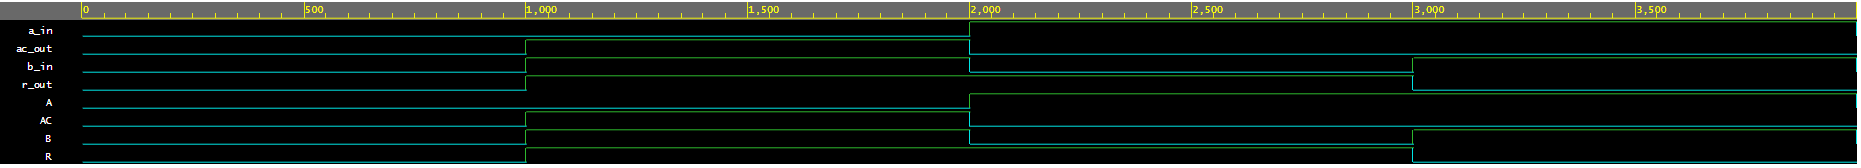
\includegraphics[width=1\textwidth]{Half Wave.png}
  \caption{Wave generated for the Half-substractor.}
  \label{fig:schematic_1}
\end{figure}
Finally, the code was synthezised and implemented in the Basys 3 board, obtaining the expected results.
\begin{figure}[H]
  \centering
  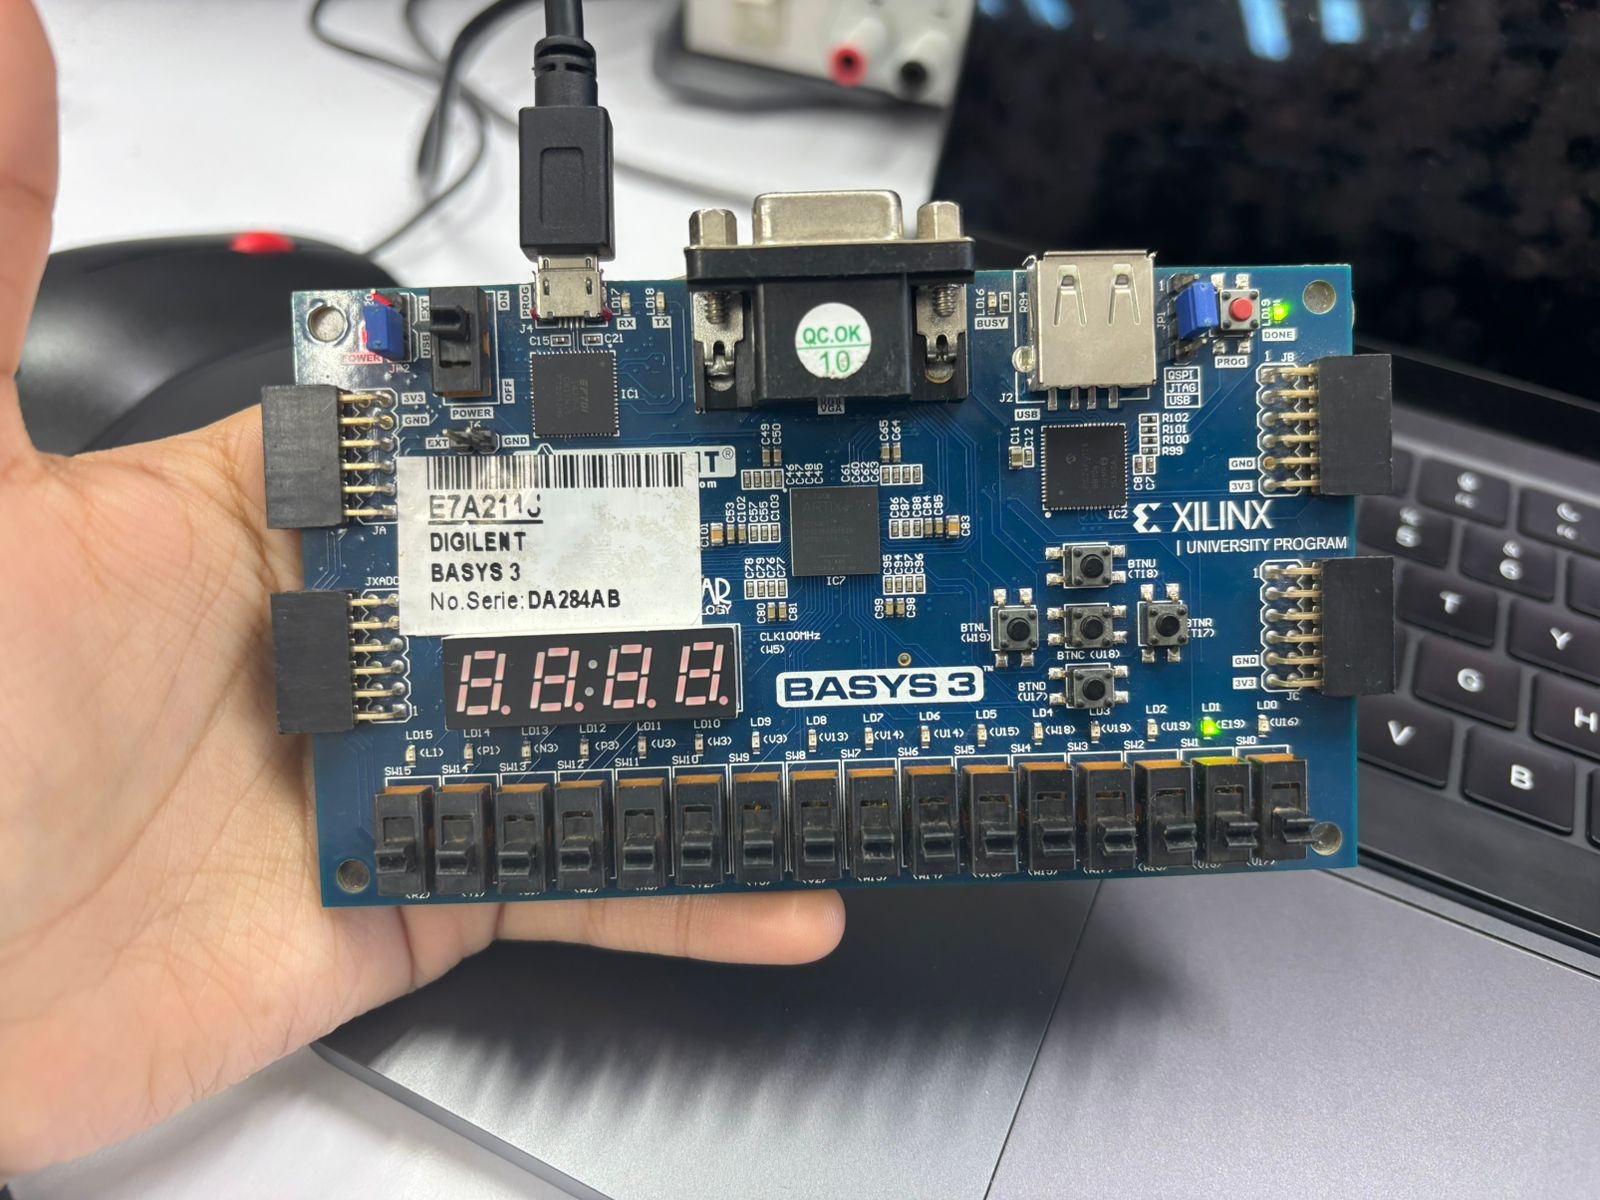
\includegraphics[width=0.4\textwidth]{HalfBasys3.jpg}
  \caption{Evidence of the functioning of the Half-substractor in the Basys 3 board.}
  \label{fig:schematic_2}
\end{figure}

\subsection{Multiplexor}
For the multiplexor, the following truth table was used to generate the EDA Code:
\begin{table}[H]
\centering
\begin{tabular}{|c|c|c|c|}
\hline
\multicolumn{3}{|c|}{\textbf{Input}} & \multicolumn{1}{c|}{\textbf{Output}} \\
\hline
\textbf{Se} & \textbf{$I_1$} & \textbf{$I_0$} & \textbf{out} \\
\hline
0 & 0 & 0 & 0 \\
0 & 0 & 1 & 1 \\
0 & 1 & 0 & 0 \\
0 & 1 & 1 & 1 \\
\hline
1 & 0 & 0 & 0 \\
1 & 0 & 1 & 0 \\
1 & 1 & 0 & 1 \\
1 & 1 & 1 & 1 \\
\hline
\end{tabular}
\caption{Truth Table for the 2-to-1 Multiplexor}
\label{tab:truth_table_mux}
\end{table}

Based on this truth table, the following Code was generated in EDA Playgrounds:
\lstinputlisting[language=VHDL,caption=Code 1: For exercise 2]{codigos/VHDL/Mult/design.vhd}
With it's appropriate testbench:
\lstinputlisting[language=VHDL,caption=Code 2: Testbench for exercise 2]{codigos/VHDL/Mult/testbench.vhd}
And, after developing the code in EDA Playgrounds, the following Wave was generating, showcasing the values of the function:

\begin{figure}[H]
  \centering
  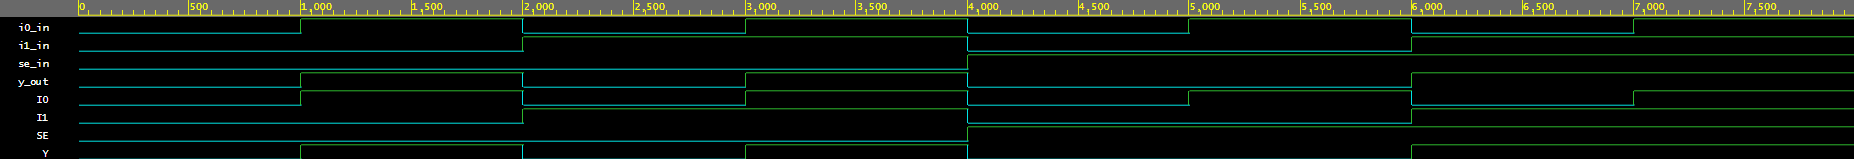
\includegraphics[width=1\textwidth]{Mult Wave.png}
  \caption{Wave generated for the Multiplexor.}
  \label{fig:schematic_3}
\end{figure}
Finally, the code was synthezised and implemented in the Basys 3 board, obtaining the expected results.
\begin{figure}[H]
  \centering
  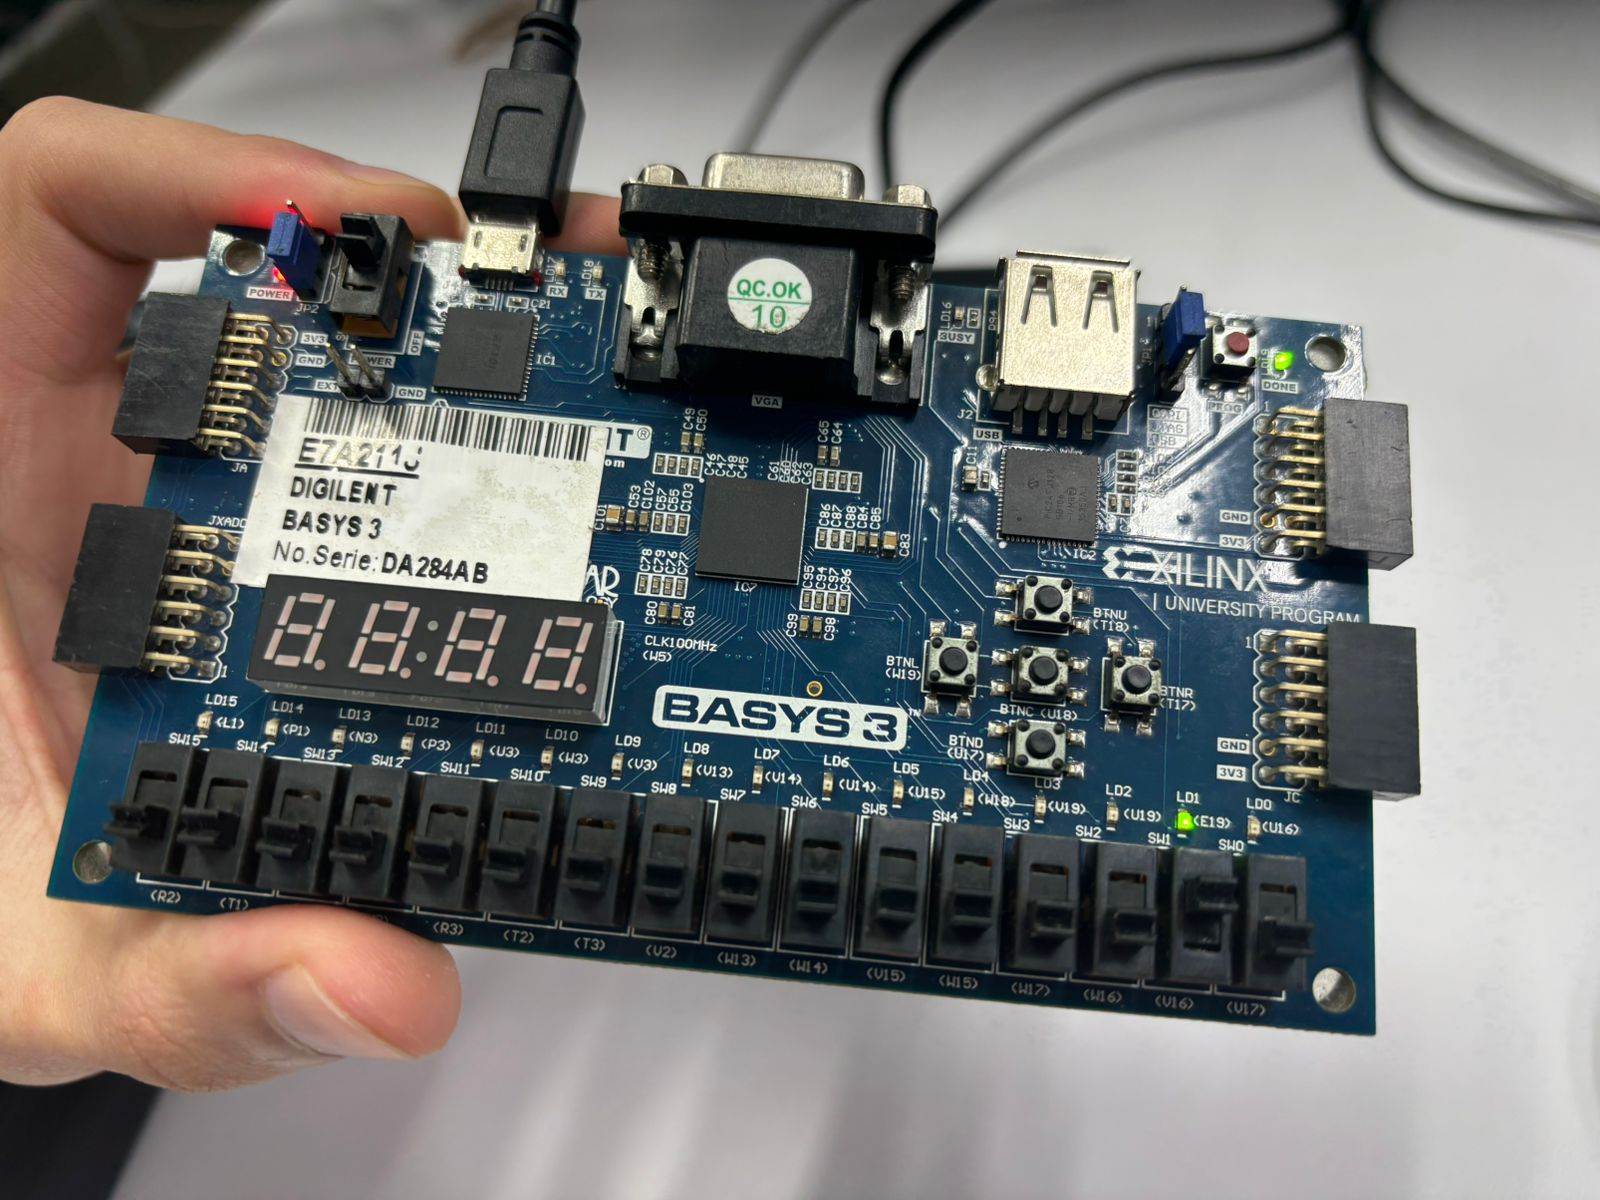
\includegraphics[width=0.4\textwidth]{MultBasys3.jpg}
  \caption{Evidence of the functioning of the Multiplexor in the Basys 3 board.}
  \label{fig:schematic_4}
\end{figure}

\subsection{Demultiplexor}
For the demultiplexor, the following truth table was used to generate the EDA Code:
\begin{table}[H]
\centering
\begin{tabular}{|c|c|c|c|}
\hline
\multicolumn{2}{|c|}{\textbf{Input}} & \multicolumn{2}{c|}{\textbf{Output}} \\
\hline
\textbf{Se} & \textbf{$I_0$} & \textbf{$O_1$} & \textbf{$O_0$} \\
\hline
0 & 0 & 0 & 0 \\
0 & 1 & 0 & 1 \\
\hline
1 & 0 & 0 & 0 \\
1 & 1 & 1 & 0 \\
\hline
\end{tabular}
\caption{Truth Table for the 1-to-2 Demultiplexor}
\label{tab:truth_table_demux_2}
\end{table}

Based on this truth table, the following Code was generated in EDA Playgrounds:
\lstinputlisting[language=VHDL,caption=Code 1: For exercise 1]{codigos/VHDL/Demult/design.vhd}
With it's appropriate testbench:
\lstinputlisting[language=VHDL,caption=Code 2: Testbench for exercise 1]{codigos/VHDL/Demult/testbench.vhd}
And, after developing the code in EDA Playgrounds, the following Wave was generating, showcasing the values of the function:

\begin{figure}[H]
  \centering
  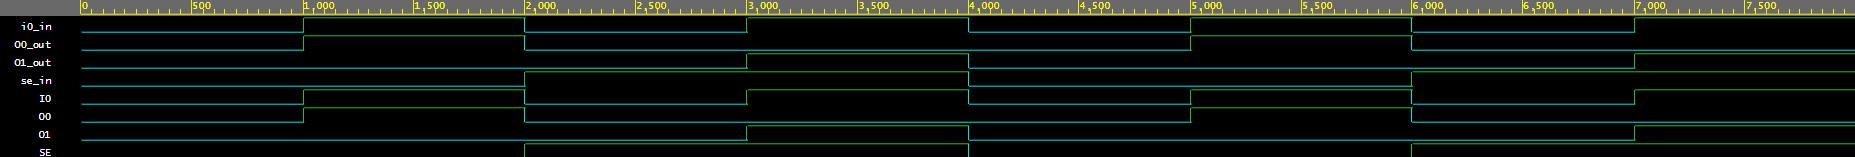
\includegraphics[width=1\textwidth]{Demult Wave.png}
  \caption{Wave generated for the Demultiplexor.}
  \label{fig:schematic_1}
\end{figure}
Finally, the code was synthezised and implemented in the Basys 3 board, obtaining the expected results.
\begin{figure}[H]
  \centering
  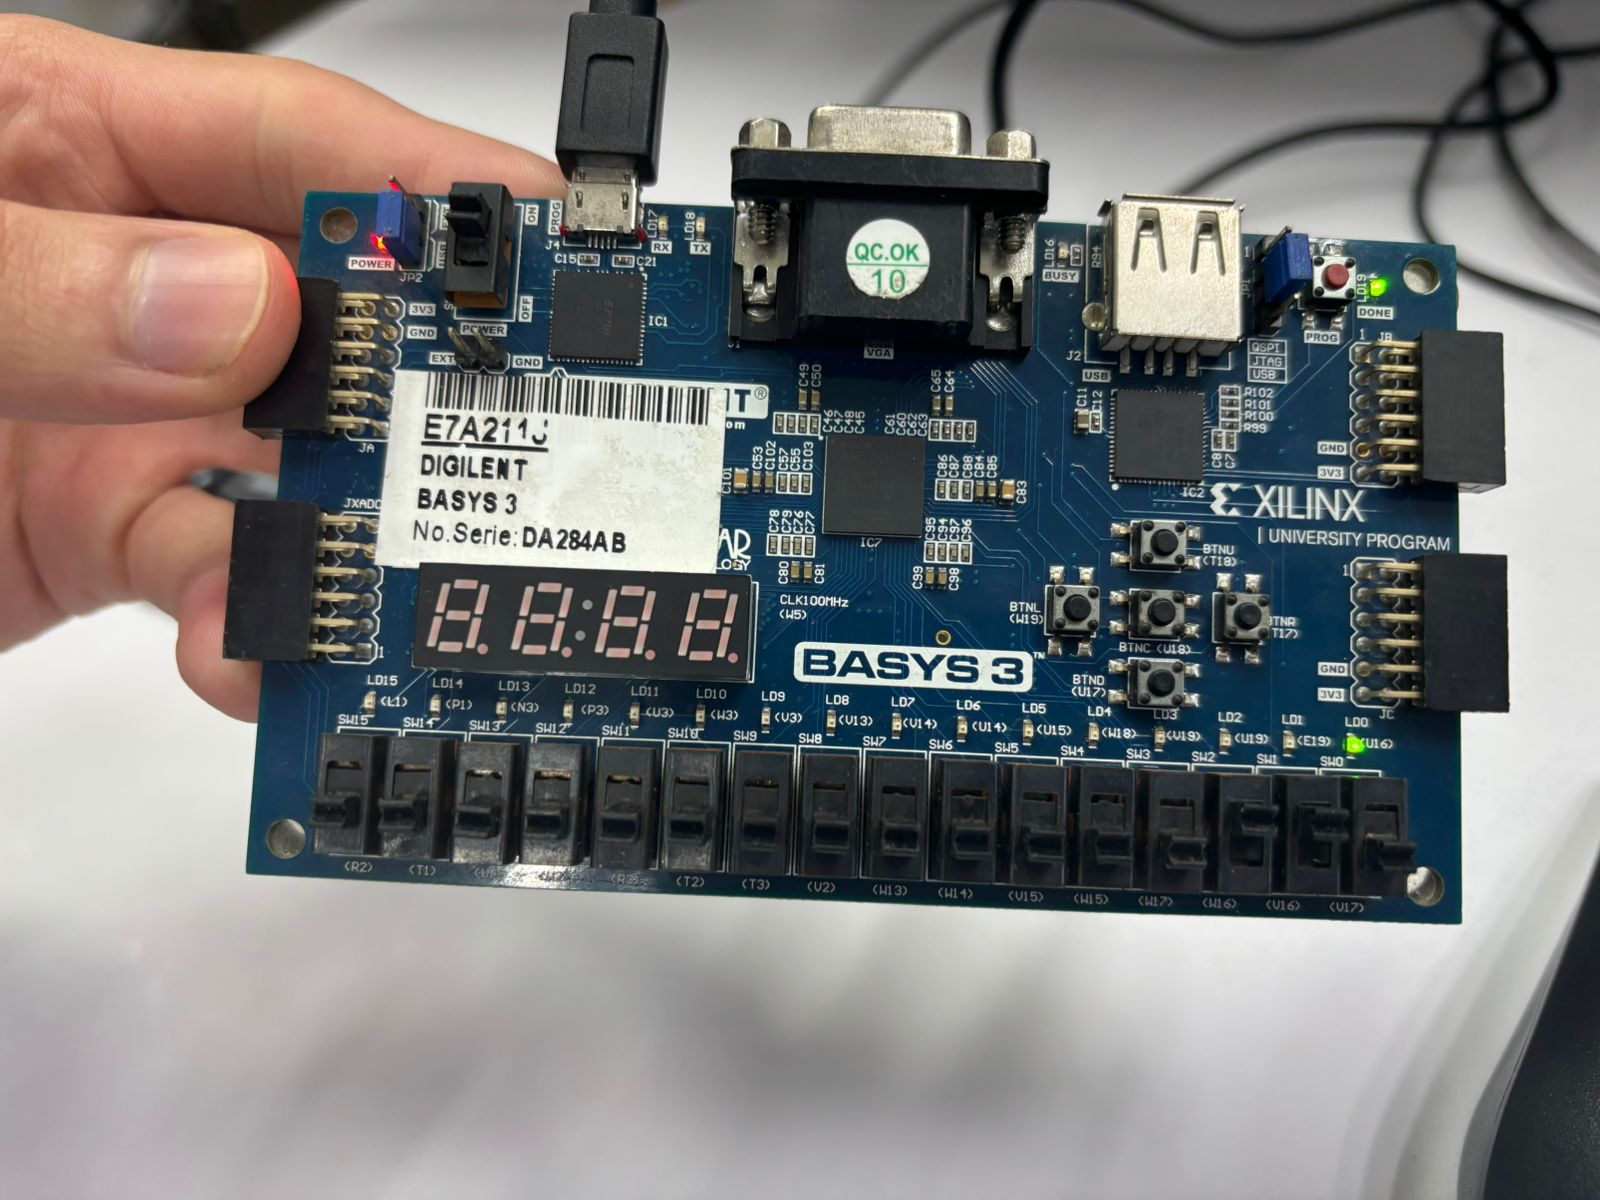
\includegraphics[width=0.4\textwidth]{DemultBasys3.jpg}
  \caption{Evidence of the functioning of the Demultiplexor in the Basys 3 board.}
  \label{fig:schematic_2}
\end{figure}

\subsection{Magnitud Comparator}
For the comparator, the following truth table was used to generate the EDA Code:
\begin{table}[H]
\centering
\begin{tabular}{|c|c|c|c|c|}
\hline
\multicolumn{2}{|c|}{\textbf{Input}} & \multicolumn{3}{c|}{\textbf{Output}} \\
\hline
\textbf{A} & \textbf{B} & \textbf{$A>B$} & \textbf{$A=B$} & \textbf{$A<B$} \\
\hline
0 & 0 & 0 & 1 & 0 \\
0 & 1 & 0 & 0 & 1 \\
1 & 0 & 1 & 0 & 0 \\
1 & 1 & 0 & 1 & 0 \\
\hline
\end{tabular}
\caption{Truth Table for a 1-bit Magnitude Comparator}
\label{tab:truth_table_comparator}
\end{table}

Based on this truth table, the following Code was generated in EDA Playgrounds:
\lstinputlisting[language=VHDL,caption=Code 1: For exercise 1]{codigos/VHDL/Comp/design.vhd}
With it's appropriate testbench:
\lstinputlisting[language=VHDL,caption=Code 2: Testbench for exercise 1]{codigos/VHDL/Comp/testbench.vhd}
And, after developing the code in EDA Playgrounds, the following Wave was generating, showcasing the values of the function:

\begin{figure}[H]
  \centering
  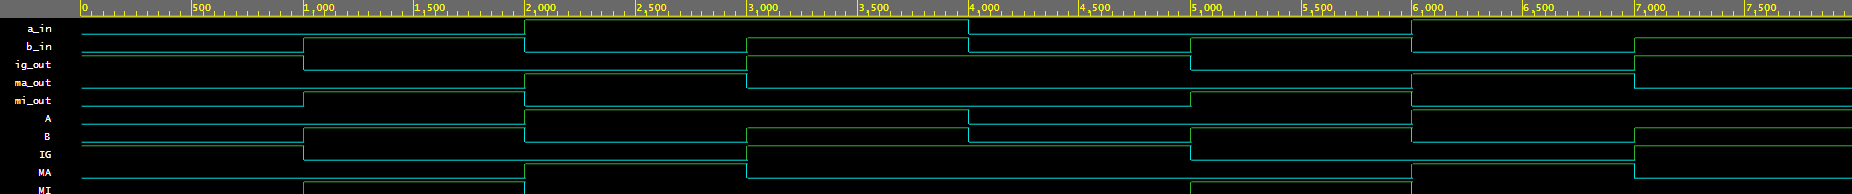
\includegraphics[width=1\textwidth]{Comp Wave.png}
  \caption{Wave generated for the Magnitud Comparator.}
  \label{fig:schematic_1}
\end{figure}
Finally, the code was synthezised and implemented in the Basys 3 board, obtaining the expected results.
\begin{figure}[H]
  \centering
  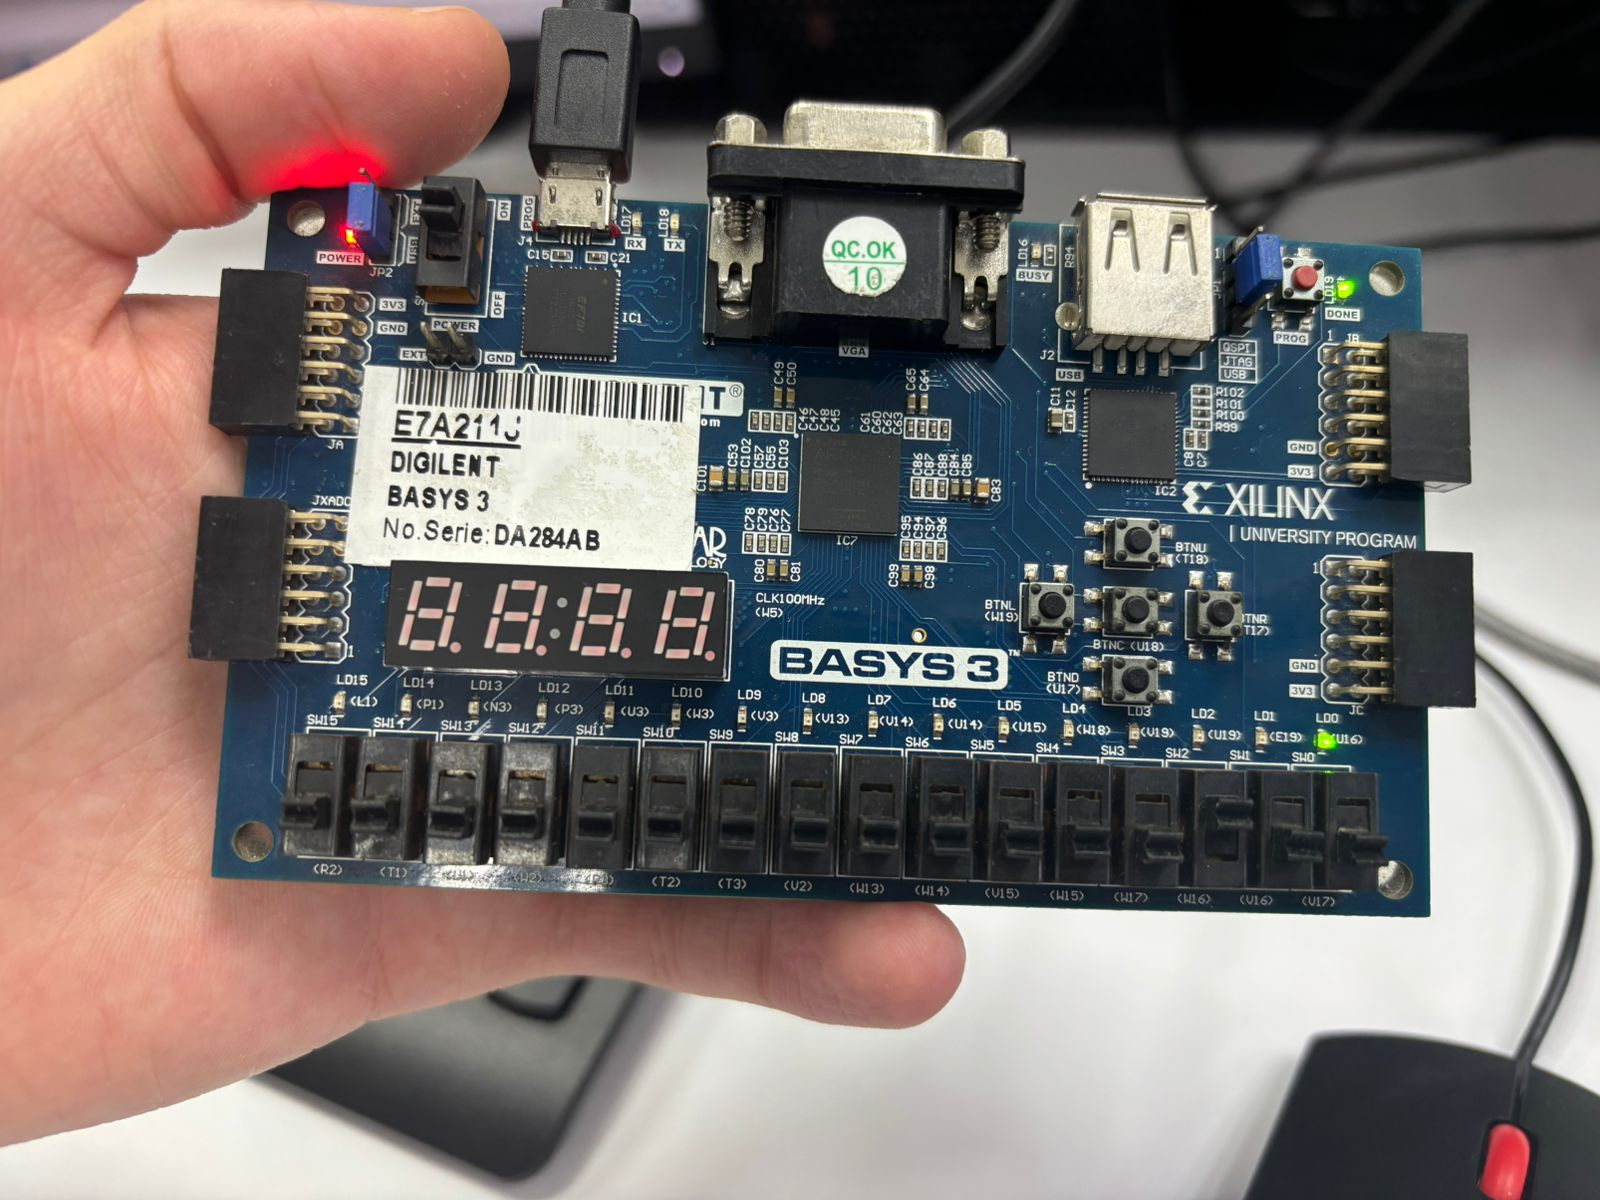
\includegraphics[width=0.4\textwidth]{CompBasys3.jpg}
  \caption{Evidence of the functioning of the Magnitud Comparator in the Basys 3 board.}
  \label{fig:schematic_2}
\end{figure}

\section{Conclusion}
This laboratory practice allowed for the analysis, simulation, and implementation of four fundamental digital circuits: half-subtractor, 2:1 multiplexer, 1$\to$2 demultiplexer, and 1-bit magnitude comparator. By comparing theoretical results, simulations in EDA Playground, and physical verification on the Basys 3 board, it was confirmed that all circuits functioned according to the intended designs.
The analysis of truth tables enabled a clear understanding of each circuit's logical behavior, while digital simulation validated the correct VHDL implementation, showing clean transitions and the absence of timing errors or interference. The Basys 3 implementation demonstrated the fidelity of the design by physically reproducing the expected operations using switches and LEDs, confirming the circuits’ stability and accuracy.
In conclusion, this practice reinforced the understanding of fundamental digital logic principles, the importance of verification through simulation, and the relevance of physical implementation to validate theoretical designs. Additionally, it strengthened skills in using digital design tools, such as EDA Playground and FPGA boards, which are essential for developing reliable and efficient digital systems.
%%%%%%% Bibliografía %%%%%%%%
\clearpage %Asegura que la bibliografía inicie en una nueva página
\bibliographystyle{bst/IEEEtran} %Estilo de bibliografía NO MODIFICAR PARA MANTENER FORMATO
\bibliography{bib/bibliografia} %Fuentes bibliográficas Se recomienda utilizar un gestor de referencias (zotero, jabref, etc..)
%%%%%%% Bibliografía %%%%%%%%      
\end{document} %Termina el documento
%% Known issues and TODO list%%%
% Warning overfull \hbox en los códigos
% Código en texto blanco y negro y comentarios en negritas => Cambiar a formato en colores